\chapter{Implementação} %não sei como chamar este capitulo
\label{chap:cap4}
Este capítulo tem por objetivo mostrar como seria uma protótipo funcional que possibilite a integração do FDR com o compilador desenvolvido nesta pesquisa através dos serviços. Na Seção \ref{sub:exper} é explicado como foi realizado o experimento através de um protótipo que integra o compilador com o verificador de modelos. Na Seção \ref{sub:results} é apresentado os resultados obtidos usando a ferramenta proposta.

\section{Experimento Realizado}
\label{sub:exper}

No Capítulo \ref{chap:cap3} foi apresentado um exemplo (Contando Caixas) adaptado de \cite{furb} que foi utilizado para exemplificar durante o processo de definição sintática e transformação. Para este experimento, vamos utilizar esse mesmo exemplo, no entanto, em sua versão completa.

%Um dos objetivos desta pesquisa é o desenvolvimento de um protótipo funcional de uma ferramenta que integre o compilador com o verificador de modelos de modo transparente ao usuário do RoboMind.
Propomos um protótipo desenvolvido em Java que provê as principais funcionalidades para a verificação automática dos programas ROBO. Implementamos uma classe chamada \texttt{RobotChecker} com três métodos. O método \texttt{translateRobo2CSP} é responsável por realizar a tradução do programa ROBO para sua a representação formal em CSP; o método \texttt{translateMap2CSP} realiza a tradução do mapa para a notação CSP; e \texttt{verifyAssertion} que faz a verificação das propriedades por meio dos serviços de FDR.

Listamos as principais funcionalidades do protótipo implementado:

\begin{itemize}
    \item Tradução de ROBO para CSP: recebe um programa ROBO como entrada e através da API do Spoofax é realizada a tradução usando o compilador desenvolvido por esta pesquisa; e como saída é gerado a especificação do programa em notação CSP.
    \item Tradução de mapa: recebe um mapa do ambiente RoboMind como entrada e realiza a tradução automática; e como saída é gerado a especificação formal em CSP do mapa.
    \item Verificação das propriedades no FDR: recebe como entrada o mapa e o programa escritos em CSP, resultado da tradução automatizada; e como saída gera os resultados das verificações e os \textit{traces} resultantes, se houver.
\end{itemize}

%\section{Definição do problema}
\label{sec:defprob}
O problema consiste em um mundo de 6 colunas e 3 linhas, onde o robô sempre inicia na primeira coluna da segunda linha e e com caixas distribuídas aleatoriamente na primeira e última linha. O objetivo é fazer o robô andar até a última coluna e mostrar alguns valores inteiros através do comando \texttt{show}. O primeiro e segundo valor representam a quantidade de caixas na primeira e última linha, respectivamente. O terceiro valor mostrado mostra quais das duas linhas possuem mais caixas: sendo o valor 1 para a primeira linha, o valor 2 para a última e valor 3 se ambas possuem a mesma quantidade. O quarto valor exibido é a diferença de caixas entre as duas linhas. O quinto e último valor, respectivamente, representa a linha na qual apareceu a primeira e última caixa: sendo valor 1 para a primeira linha; valor 2 para a segunda; e valor 3 para ambas. Para ilustrar o experimento, considere os mapas apresentados na Figura \ref{fig:problem}, para cada um dos mapas tem-se a saída esperada no término da execução do programa.

\begin{figure}[h]
\centering
\caption{Mapas e saídas esperadas do problema ``Contando Caixas"}
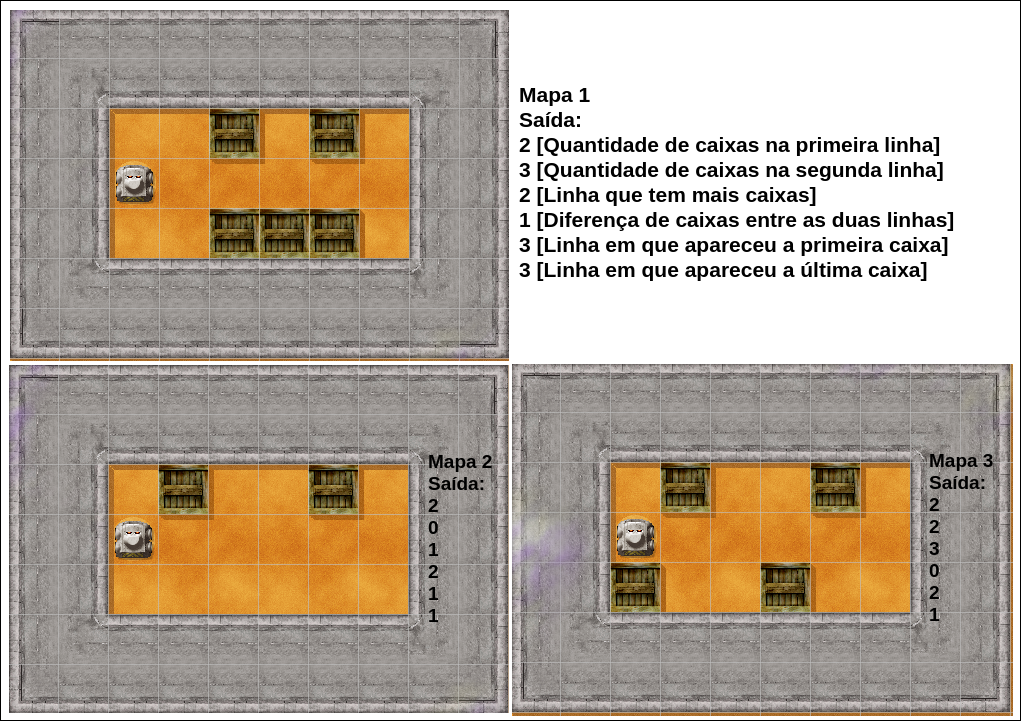
\includegraphics[height=10cm]{figuras/problema.png}
\fonte{\cite{furb}}
\label{fig:problem}
\end{figure}

Apresentado o problema, o próximo passo foi desenvolver uma solução para esse problema. Então desenvolvemos um programa ROBO capaz de apresentar as mesmas saídas para cada um desses mapas. A solução que propusemos contém cinco procedimentos e algumas variáveis que são suficientes para resolver o problema em questão. A Figura \ref{fig:solution} apresenta um trecho do código ROBO proposto. Podemos notar que há uma estrutura de repetição (\texttt{repeatWhile}) com uma condição (\texttt{frontIsClear}) que verifica se a célula posterior ao robô está livre. Os cinco procedimentos definidos são: (1) \texttt{countLeft}, conta a quantidade de caixas à esquerda do robô; (2) \texttt{countRight}, conta a quantidade de caixas à direita do robô; (3) \texttt{showsMoreBoxes}, mostra qual linha tem mais caixas e a diferença entre elas; (4) \texttt{getBoxsFirstLine}, mostra a quantidade de caixas na primeira linha; por fim, (5) \texttt{getBoxLastLine}, mostra a quantidade de caixas na última linha.

\begin{figure}[h]
\centering
\caption{Solução proposta em ROBO para o problema Contando Caixas}
\lstinputlisting{codes/solution.rob}
\fonte{O autor}
\label{fig:solution}
\end{figure}

Para validar a efetividade do compilador integrado ao FDR, foi necessário verificar as saídas geradas pelo protótipo e executar os \textit{traces} no ambiente RoboMind, obtidos através do resultado da verificação da propriedade: \texttt{assert PROGRAM :[deadlock free [F]]}. Na próxima seção estão descritos os resultados gerados pela ferramenta.

Definimos três testes, um para cada mapa. Na Tabela \ref{table:map1} estão dispostas as entradas e saídas geradas após a execução de cada método. Para o método \texttt{translateRobo2CSP} o arquivo \texttt{program.robo} (o mesmo da Figura \ref{fig:solution}) e  como saída obtivemos o arquivo \texttt{program.csp} com a especificação formal do programa ROBO.

\begin{table}
\caption{Entradas e saídas para o mapa 1}
\resizebox{\textwidth}{!}{%
\begin{tabular}{*{14}{|c}|}
\hline
\multicolumn{3}{|c|}{\textbf{Map 1}} \\ \hline
\textbf{method} & \textbf{input} & \textbf{output} \\ \hline
translateRobo2CSP & program.robo & program.csp \\ \hline
translateMap2CSP & map1.map & map1.csp \\ \hline
verifyAssertion & program.csp, map1.csp, test1\_program\_map1.csp & result1, traces1 \\ \hline
\end{tabular}%
}
\label{table:map1}
\fonte{O autor}
\end{table}

\begin{table}[]
\label{tab:map2}
\caption{Entradas e saídas para o mapa 2}
\resizebox{\textwidth}{!}{%
\begin{tabular}{*{14}{|c}|}
\hline
\multicolumn{3}{|c|}{\textbf{Map 2}} \\ \hline
\textbf{method} & \textbf{input} & \textbf{output} \\ \hline
translateRobo2CSP & program.robo & program.csp \\ \hline
translateMap2CSP & map2.map & map2.csp \\ \hline
verifyAssertion & program.csp, map2.csp, test2\_program\_map2.csp & result2, traces2 \\ \hline
\end{tabular}%
}
\fonte{O autor}
\end{table}

\begin{table}[]
\label{tab:map3}
\caption{Entradas e saídas para o mapa 3}
\resizebox{\textwidth}{!}{%
\begin{tabular}{*{14}{|c}|}
\hline
\multicolumn{3}{|c|}{\textbf{Map 3}} \\ \hline
\textbf{method} & \textbf{input} & \textbf{output} \\ \hline
translateRobo2CSP & program.robo & program.csp \\ \hline
translateMap2CSP & map3.map & map3.csp \\ \hline
verifyAssertion & program.csp, map3.csp, test3\_program\_map3.csp & result3, traces3 \\ \hline
\end{tabular}%
}
\fonte{O autor}
\end{table}

\section{Resultados}
\label{sub:results}
...
\begin{table}[]
\caption{Resultado obtido após a verificação do FDR}
\resizebox{\textwidth}{!}{%
\begin{tabular}{*{14}{|c}|}
\multicolumn{1}{c}{Map 1} & \multicolumn{1}{c}{Map 2} & \multicolumn{1}{c}{Map 3} \\
assert PROGRAM :{[}deadlock free {[}F{]}{]} & assert PROGRAM :{[}deadlock free {[}F{]}{]} & assert PROGRAM :{[}deadlock free {[}F{]}{]} \\
Result: Failed & Result: Failed & Result: Failed \\
Counterexample - Traces: & Counterexample - Traces: & Counterexample - Traces: \\
right() & right() & right() \\
forward(1) & forward(1) & forward(1) \\
forward(1) & forward(1) & forward(1) \\
forward(1) & forward(1) & forward(1) \\
forward(1) & forward(1) & forward(1) \\
forward(1) & forward(1) & forward(1) \\
show(2) & show(2) & show(2) \\
show(3) & show(0) & show(2) \\
show(2) & show(1) & show(3) \\
show(1) & show(2) & show(0) \\
show(3) & show(1) & show(2) \\
show(3) & show(1) & show(1)
\end{tabular}%
}
\fonte{O autor}
\end{table}

Levando-se em conta o que foi observado, para os três mapas analisados, comparando as saídas geradas pelo RoboMind e pela ferramenta proposta, é notório que a tradução do programa foi realizado corretamente, isto é, os programas CSP são representados semanticamente equivalentes a ROBO.


